\chapter{Readme-file of the backend-solution}
\label{app:backend-readme}
In the git-repository on GitHub, there is a \code{readme}-file in which the team explains the workflow to anyone who wants to contribute, the general structure of the project as well as how to get the project running locally or in a production environment.The file can be found online at \url{https://github.com/CrowdShelf/server/blob/dev/README.md}, or below.


%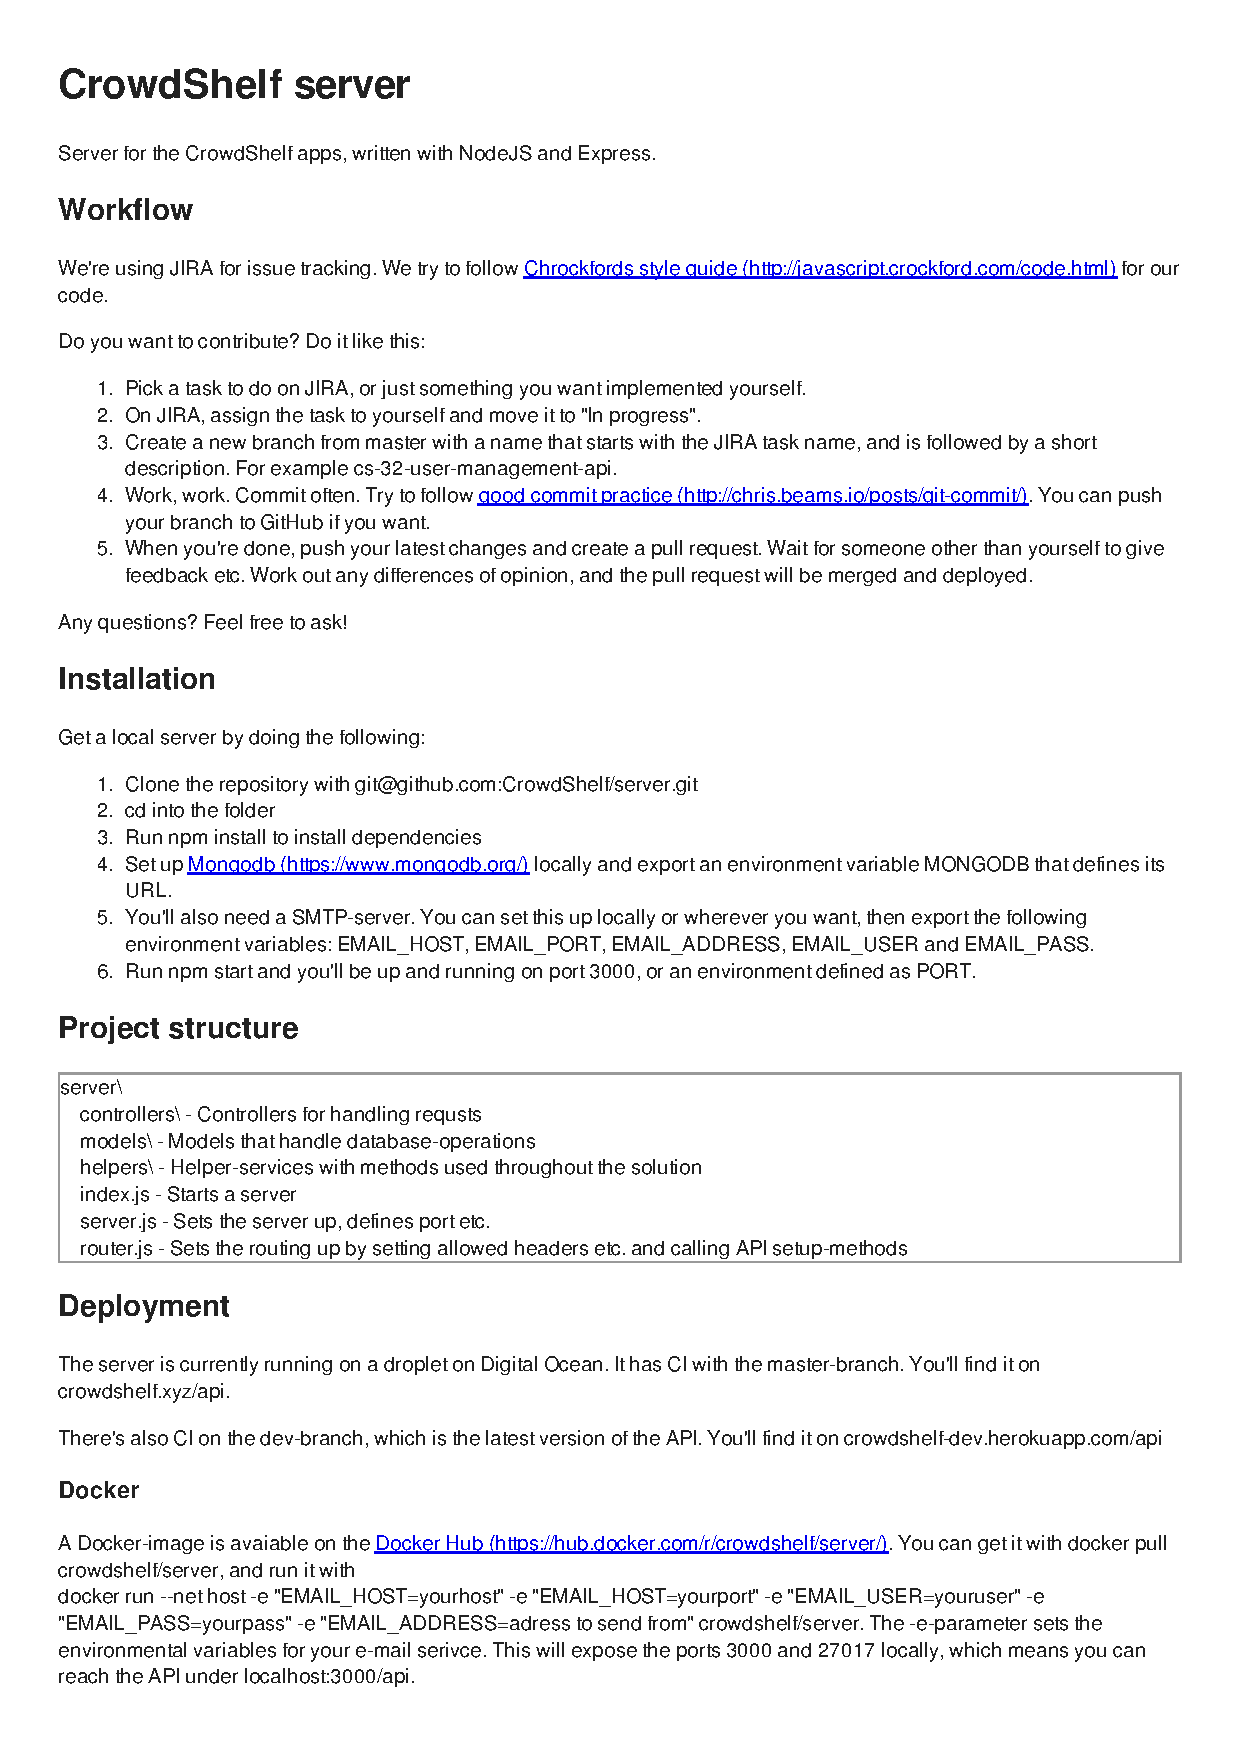
\includepdf[scale=0.8,pages={-},pagecommand=\chapter{Readme-file of the backend-solution}]{appendices/backend-README.pdf}

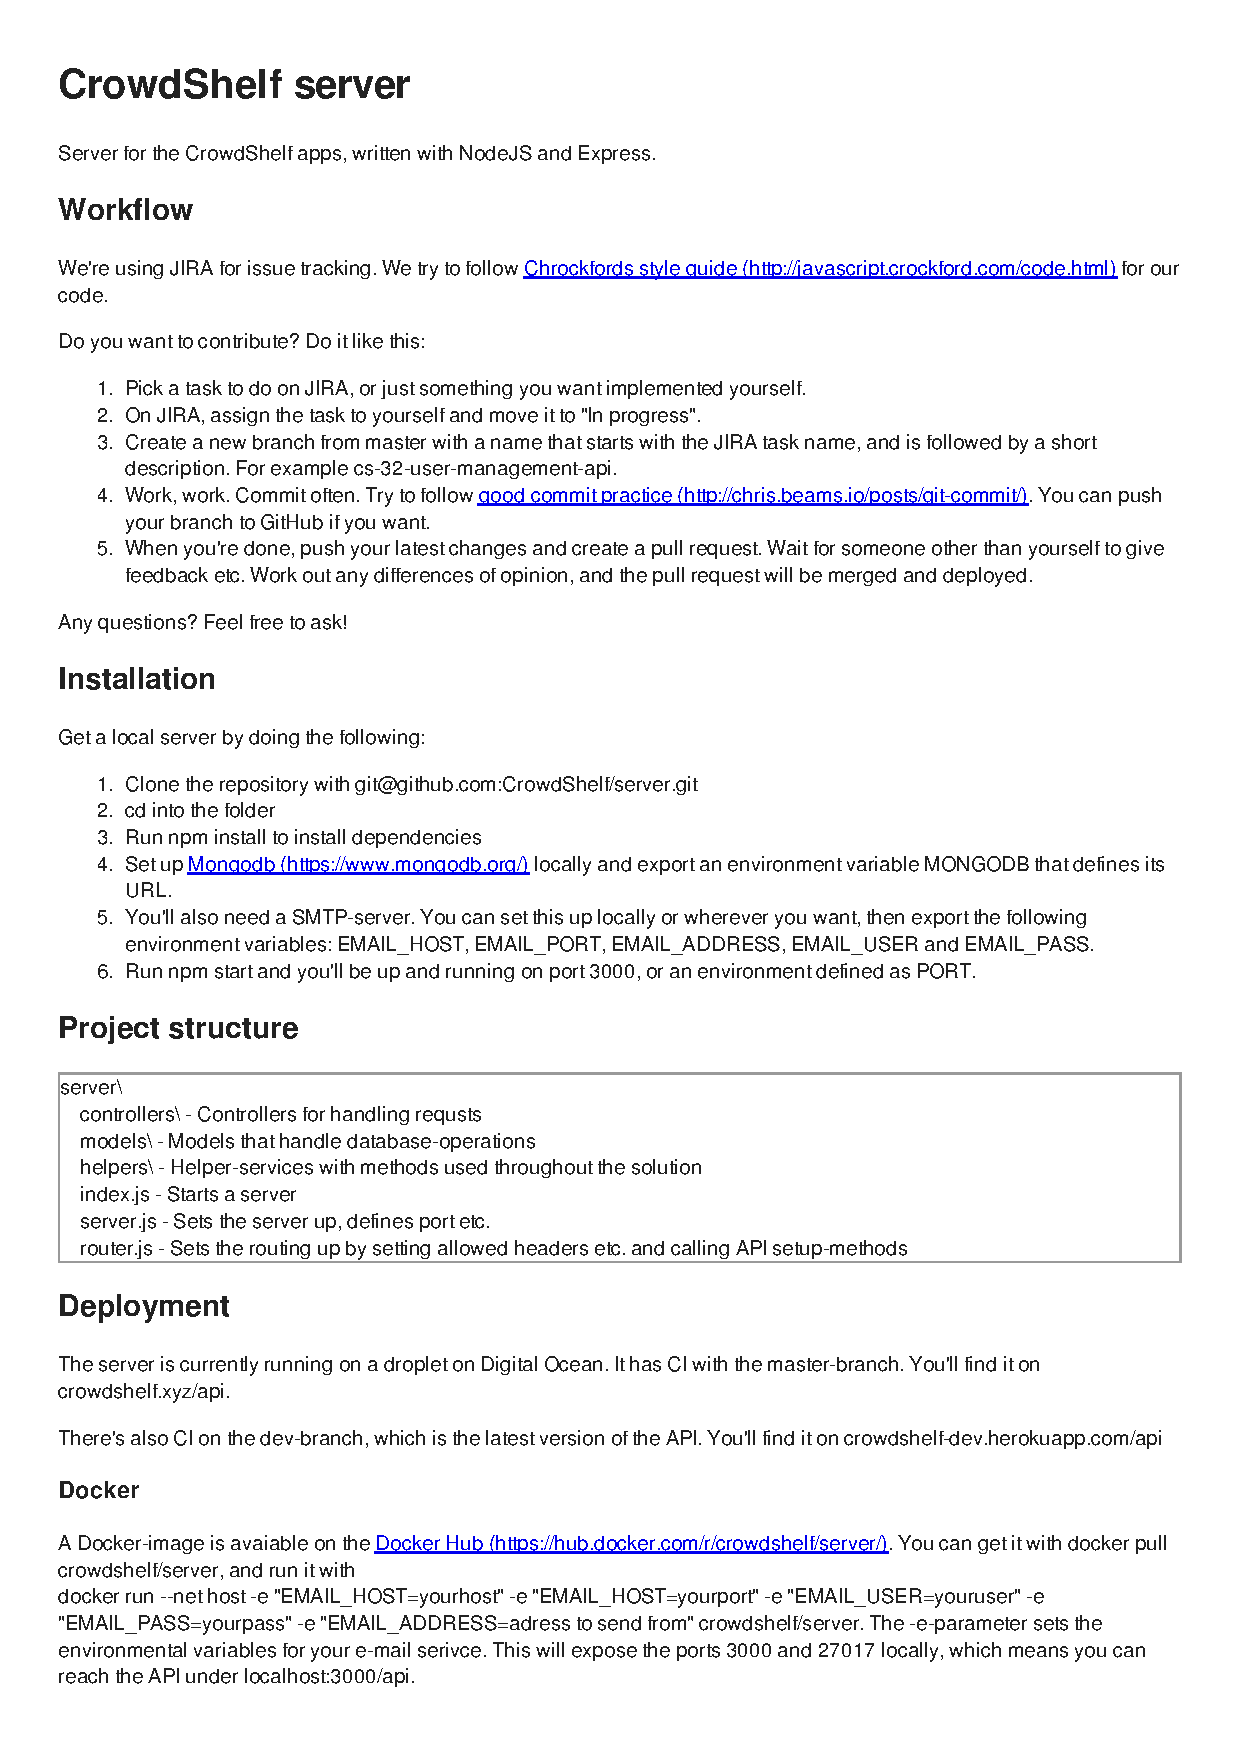
\includepdf[pages={-},fitpaper=true]{appendices/backend-README.pdf}

